\section{How to write graph states, XOR-states and stabilizer states as Tower-\limdds}
\label{sec:graph-states-limdds}
\label{sec:proof-stabilizer-states-tower-limdds}
%\todo[inline]{Tim: should add `semi-reduced' to all three theorems? (even though this is only properly defined in the context of Pauli-\limdds?)}
%\todo[inline]{Tim: not yet made domain notation correct, e.g. make all Pauli strings represented by $P, Q$, etc.}

In this appendix, we prove that the families of $\langle Z\rangle$-, 
$\langle X\rangle$-, and Pauli-Tower-\limdds correspond to graph states, XOR states (see \autoref{def:xor-states} below), and stabilizer states, respectively, in \autoref{thm:graph-states-z-limdd}, \autoref{lemma:vector-space-x-limdd} and \autoref{thm:pauli-tower-limdds-are-stabilizer-states} below.
\autoref{def:reduced-limdd} for reduced \Pauli-\limdds also holds when exchanging \Pauli{} with $\bracket{X}$. However, it does not work for $\bracket{Z}$ by \ref{obs:subgroups}. Note however, that our proofs do not rely on the reduced definition, but on \autoref{def:limdd}.


We recall that a Tower-\limdd representing an $n$-qubit state is a \limdd which has, besides the leaf, $n$ nodes.
%Graph states and XOR states are stabilizer states, so they can be succintly represented by a generating set of their stabilizer groups.
%Our proofs are constructive: given the generating set for a graph state/XOR state/stabilizer state, we construct the state's $\langle Z \rangle$-/$\langle X\rangle$-/$\Pauli$-Tower-\limdds in polynomial time in the number of qubits.

\begin{proposition}[Graph states are $\langle Z\rangle$-Tower-\limdds]
    \label{thm:graph-states-z-limdd}
    Let $n\geq 1$.
    Denote by $\mathcal{G}_n$ the set of $n$-qubit graph states and write $\mathcal{Z}_n$ for the set of $n$-qubit quantum states which are represented by Tower-\limdds which low-edge-labels $\id$ and high-edge labels $\lambda \bigotimes_j P_j$ with $P_j \in \{\id[2], Z\}$ and $\lambda \in \{0, 1\}$.
    Then $\mathcal{G}_n = \mathcal{Z}_n$.
\end{proposition}
\begin{proof}
    We establish $\mathcal{G}_n \subseteq \mathcal{Z}_n$ by providing a procedure to convert any graph state in $\mathcal{G}_n$ to a reduced Tower-\limdd in $\mathcal{Z}_n$.
	See \autoref{fig:graph-state-as-line-iso-qmdd} for an example of a $4$-qubit graph state.
	
	\textbf{Base case: $n=1$.} We note that there is only one single-qubit graph state by definition (see \autoref{eq:graph-state-definition}), which is \mbox{$\ket{+} := (\ket{0} + \ket{1}) / \sqrt{2}$} and can be represented as \limdd by a single node (in addition to the leaf node): see \autoref{fig:graph-state-as-line-iso-qmdd}(a).
	
	\textbf{Induction case.}For the inductive step, we consider an $(n+1)$-qubit graph state $\ket{G}$ corresponding to the graph~$G$.
	We isolate the $(n+1)$-th qubit by decomposing the full state definition from  \autoref{eq:graph-state-definition} according to \autoref{eq:quantum-state-recursive}:
	\begin{equation}
	% Overweeg: 
        \ket{G} = 
        \frac{1}{\sqrt{2}}\left(\ket{0} \otimes \ket{G_{1..n}} + \ket{1} \otimes 
            \underset{\textnormal{Isomorphism B}}{ \underbrace{
\left[
            \bigotimes_{(n+1,j)\in E} Z_j
            \right] 
            }}
        \ket{G_{1..n}}\right)
		\label{eq:graph-state-induction}
	\end{equation}
where $E$ is the edge set of $G$ and $G_{1..n}$ is the induced subgraph of $G$ on vertices $1$ to $n$.
Thus, $\ket{G_{1..n}}$ is an $n$-qubit graph state on qubits 1 to $n$.
% Can be represented as <<a>> line-like \limdd
    Since $\ket{G_{1..n}}$ is a graph state on $n$ qubits, by the induction hypothesis, we have a procedure to convert it to a Tower-\limdd $\in \mathcal{Z}_{n-1}$.
Now we construct a Tower-\limdd for $\ket{G}$ as follows.
The root node has two outgoing edges, both going to the node representing $\ket{G_{1.. n}}$.
    The node's low edge is labeled with $\mathbb I$, and the node's high edge is labeled $B=0$ if the $(n+1)$-th qubit is isolated, and otherwise with 
\begin{align}
	B = \bigotimes_{(n+1,j)\in E}Z_j
\end{align}
Thus the root node represents the state $\ket{0}\ket{G_{1..n}}+\ket{1}B\ket{G_{1..n}}$, satisfying \autoref{eq:graph-state-induction}.
\begin{figure*}
    \begin{centering}
    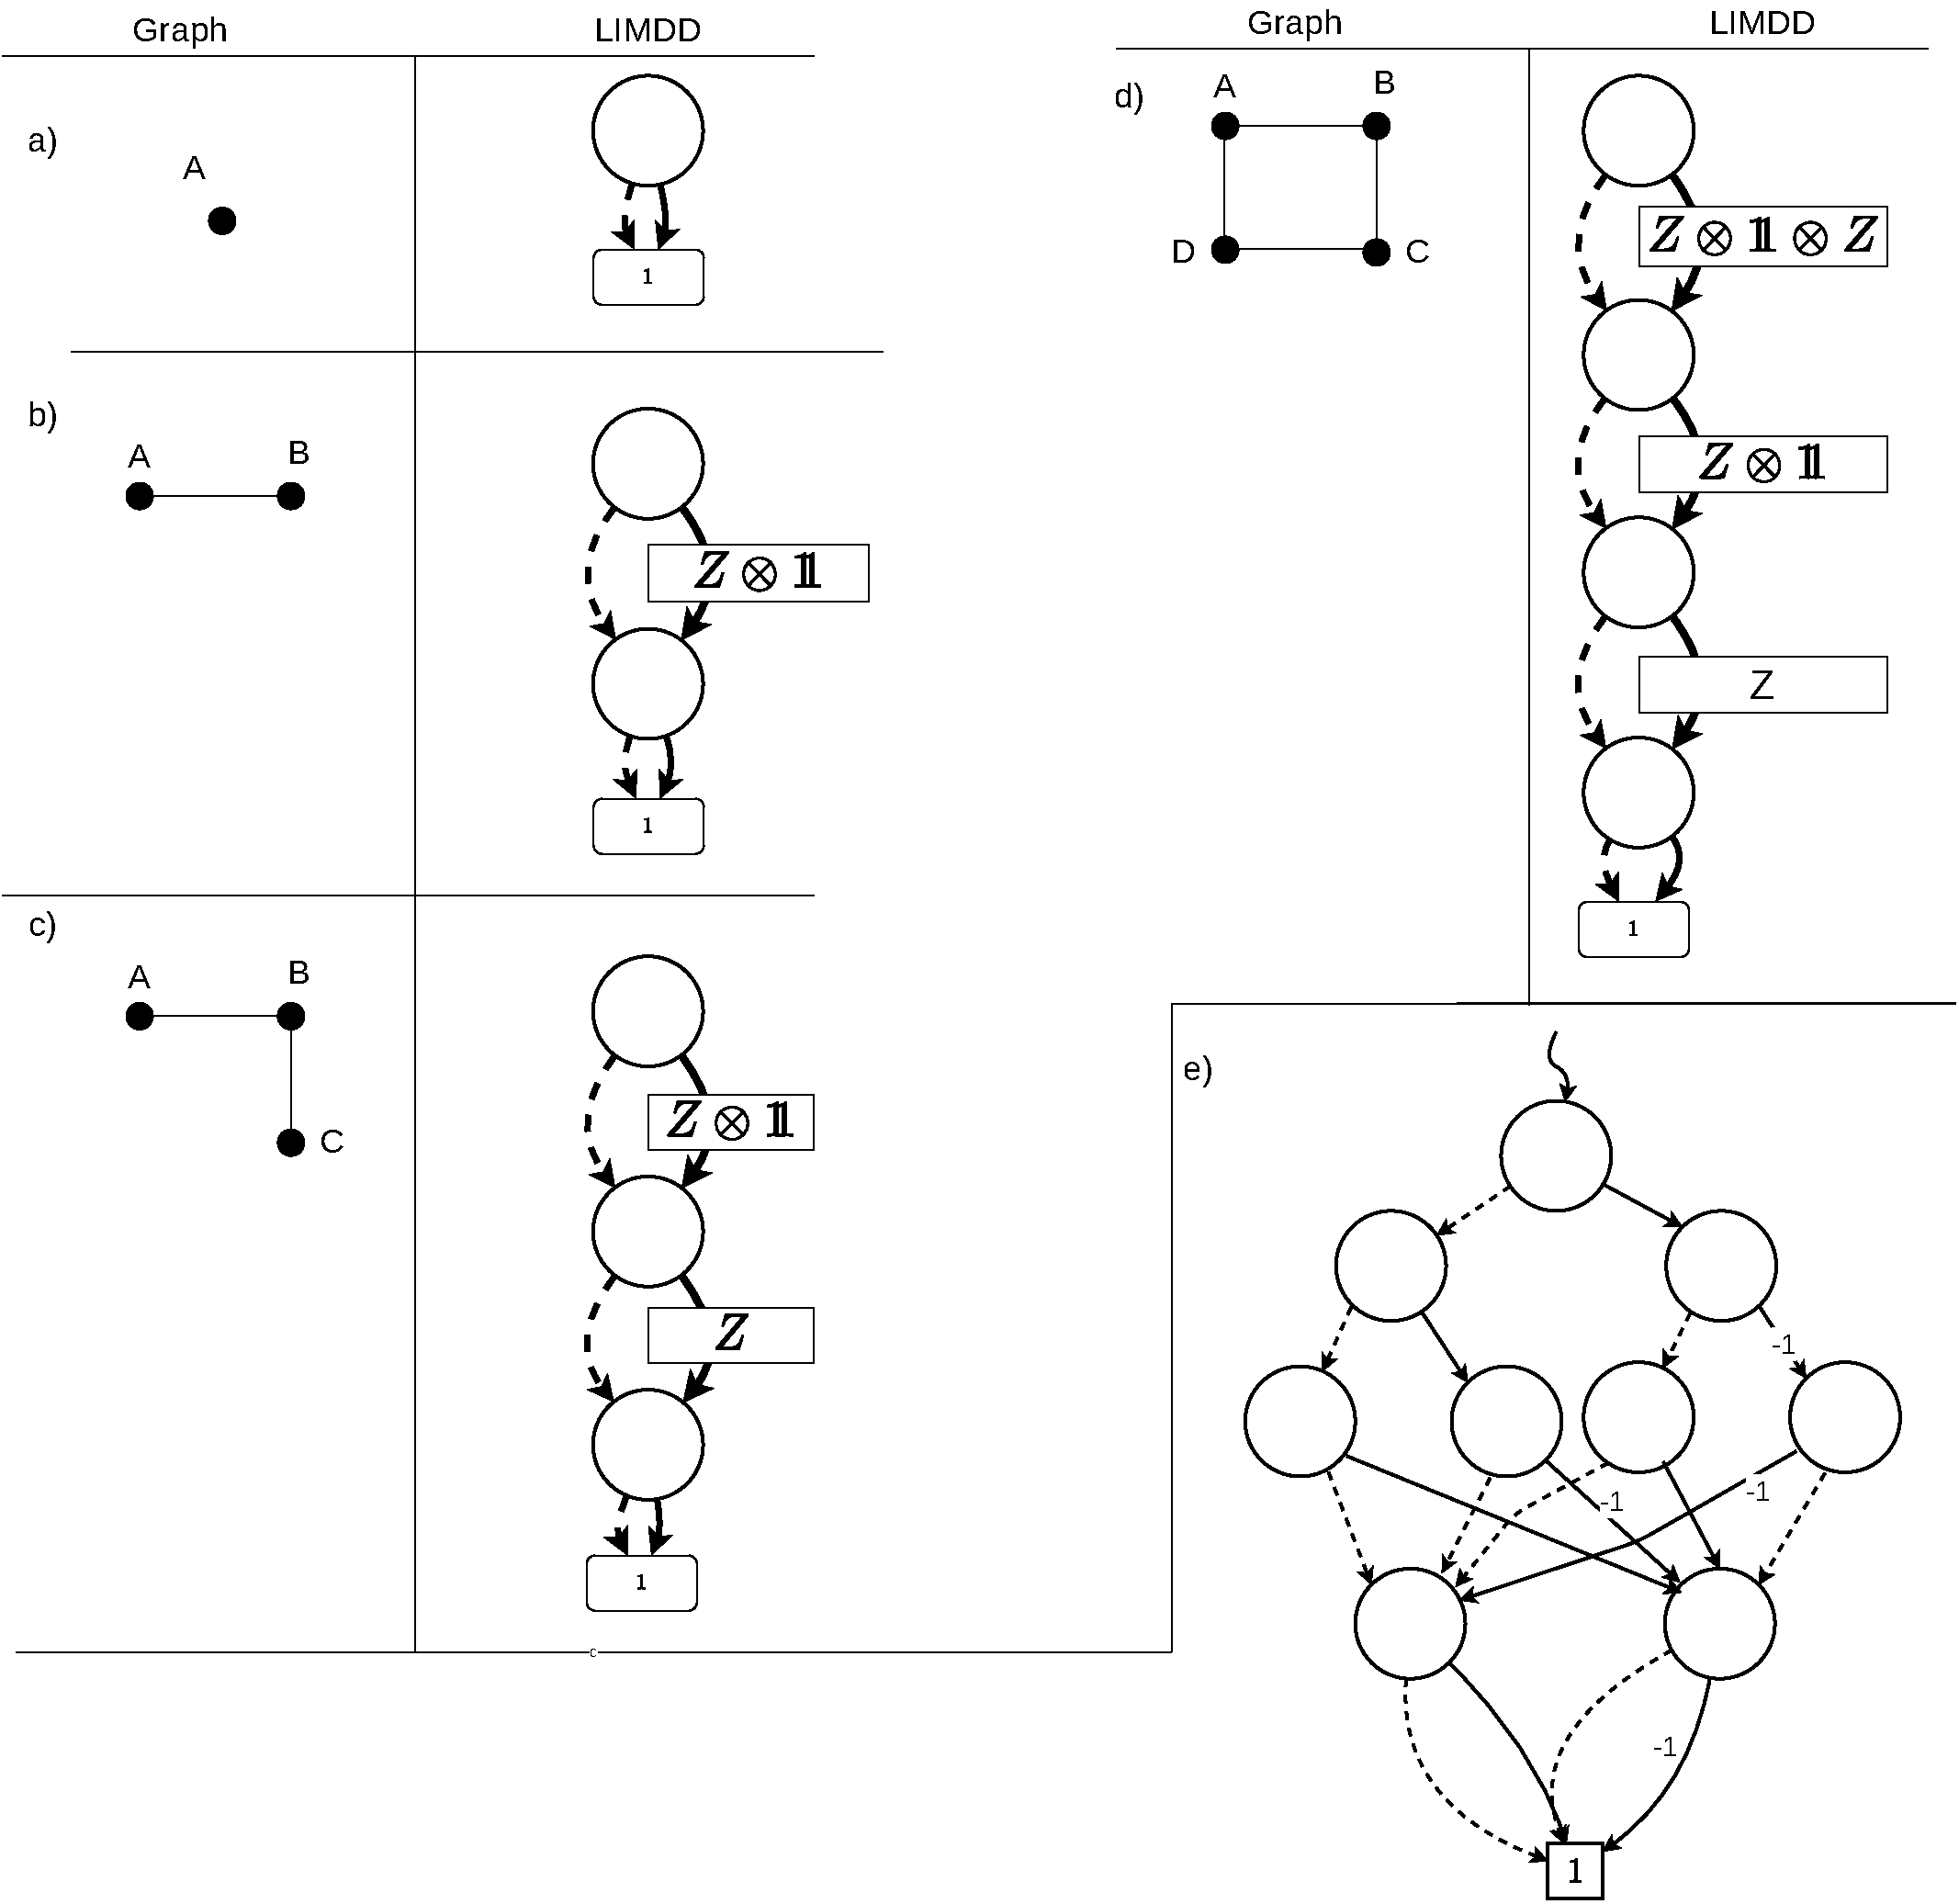
\includegraphics[width=1.0\textwidth]{pics/graph-state-construction.pdf}
	\caption{
		Construction of the Tower-\limdd for the 4-qubit cluster graph state, by iterating over the number of vertices in the graph.
    (a) First, we consider the single-qubit graph state, which corresponds to a the subgraph containing only vertex $A$.
    (b) Then, we add vertex $B$, which is connected to $A$ by an edge.
	The resulting \limdd is constructed from the \limdd from (a) by adding a new root node and an isomorphism node.
	The isomorphism is $\unit_A \otimes Z_B$, since vertex $C$ is connected to vertex $B$ (yielding the $Z$ operator) but not to $A$ (yielding the identity operator $\unit$).
    This process is repeated for a third vertex $C$ (c) until we reach the \limdd of the full 4-qubit cluster graph state (d).
	For comparison, (e) depicts a QMDD for the same graph state, which has width 4 instead of 1 for the \limdd.
		\label{fig:graph-state-as-line-iso-qmdd}
		}
    \end{centering}
\end{figure*}


    To prove $\mathcal{Z}_n \subseteq \mathcal{G}_n$, consider the fact that the reverse algorithm is simply the interpretation of the resulting root node $\ket v$ (see semantics in \autoref{def:limdd}).
A simple counting argument based on the above construction shows that $\sizeof{\mathcal{Z}_n} = \sizeof{\mathcal{G}_n} = 2^{n \choose 2}$, so the conversion is indeed a bijection.
\end{proof}


We now define ``XOR-states'' and prove that they are represented exactly by Tower-$\braket{X}$-\limdds.

\begin{definition}[XOR state]
	Let $V\subseteq\{0,1\}^n$ be a vector space over $\{0,1\}$, i.e., $V$ is not empty and it holds that $u,v\in V$ implies $u\oplus v\in V$.
	Then the following quantum state is the corresponding XOR state,
	\begin{align}
		\ket{S} = \frac{1}{\sqrt{|S|}}\sum_{x\in S}\ket{x}
	\end{align}
\end{definition}

\begin{proposition}[XOR-states are $\langle X\rangle$-Tower-\limdds]
    \label{lemma:vector-space-x-limdd}
    Let $n\geq 1$.
    Denote by $\mathcal{V}_n$ the set of $n$-qubit XOR states and write $\mathcal{X}_n$ for the set of $n$-qubit quantum states which are represented by Tower-\limdds with low edge labels $\id$ and high edge labels $\lambda \bigotimes_j P_j$ with $P_j \in \{\mathbb I, X\}$ and $\lambda \in \{0, 1\}$.
    Then $\mathcal{V}_n = \mathcal{X}_n$.
\end{proposition}
\begin{proof}
    We prove $\mathcal{V}_n \subseteq \mathcal{X}_n$ by providing a procedure for constructing a Tower-\limdd for an XOR-state.
    The procedure is recursive on the number of qubits.

	\textbf{Base case: $n=1$.} In this case, there are two XOR states: $\ket{0}$ and $(\ket{0} + \ket{1}) / \sqrt{2}$, which are represented by a single node which has a low and high edge pointing to the leaf node with low/high edge labels 1/0 and 1/1, respectively.
	
	\textbf{Induction case. }Now consider an $(n+1)$-qubit XOR state $\ket{S}$ for a vector space $S\subseteq \{0,1\}^{n+1}$ for some $n\geq 1$ and assume we have a procedure to convert any $n$-qubit XOR state into a Tower-\limdd~in~$ \mathcal{X}_n$. 
We consider two cases, depending on whether the first bit of each element of $S$ is zero:
    \begin{enumerate}[(a)]
        \item{
                The first bit of each element of $S$ is $0$.
                Thus, we can write $S = \{0x \mid  x \in S_0\}$ for some set $S_0\subseteq\{0, 1\}^n$.
            Then $0a,0b\in S \implies 0a\oplus 0b\in S$ implies $a,b\in S_0 \implies a\oplus b\in S_0$ and thus $S_0$ is an length-$n$ bit string vector space.
            Thus by assumption, we have a procedure to convert it to a Tower-\limdd in $\mathcal{X}_n$.
            Convert it into a Tower-\limdd in $\mathcal{X}_{n+1}$ for $\ket{S}$ by adding a fresh node on top with low edge label $\id[2]^{\otimes n}$ and high edge label $0$, both pointing to the the root $S$.
            }
         \item{
                 There is some length-$n$ bit string $u$ such that $1u\in S$.
                 Write $S$ as the union of the sets $\{0x \mid x \in S_0\}$ and $\{1x \mid x\in S_1\}$ for sets $S_0, S_1 \subseteq \{0,1\}^n$.
                 Since $S$ is closed under element-wise XOR, we have $1u \oplus 1x = 0(u\oplus x) \in S$ for each $x\in S_1$ and therefore $u\oplus x \in S_0$ for each $x \in S_1$.
                 This implies that $S_1 = \{u\oplus x\mid x\in S_0\}$ and thus $S$ is the union of $\{0x \mid  x \in S_0\}$ and $\{1u \oplus 0x\mid x\in S_0\}$.
                 By similar reasoning as in case (a), we can show that $S_0$ is a vector space on length-$n$ bit strings.
                 
                 We build a Tower-\limdd for $\ket S$ as follows.
                 By the induction hypothesis, there is a Tower-\limdd with root node $v$ which represents $\ket{v}=\ket{S_0}$.
                 We construct a new node whose two outgoing edges both go to this node $v$.
                 Its low edge has label $\id[2]^{\otimes n}$ and its high edge has label $P=P_n\otimes\cdots\otimes P_1$ where $P_j=X$ if $u_j=1$ and $P_j=\mathbb I$ if $u_j=0$.
             }
    \end{enumerate}

	We now show $\mathcal{V}_n\subseteq \mathcal X_n$, also by induction.
	
	\textbf{Base case: $n=1$.} There are only two Tower-\limdds on $1$ qubit satisfying the description above, namely
	\begin{enumerate}[(1)]
		\item A node whose two edges point to the leaf. Its low edge has label $1$, and its high edge has label $0$.
		This node represents the XOR state $\ket 0$, corresponding to the vector space $V=\{0\}\subseteq\{0,1\}^1$.
		\item A node whose two edges point to the leaf. Its low edge has label $1$ and its high edge also has label $1$.
		This node represents the XOR state $\ket 0+\ket 1$, corresponding to the vector space $V=\{0,1\}$.
	\end{enumerate}
	
	\textbf{Induction case. } Let $v$ be the root node of a Tower-\limdd as described above.
	We distinguish two cases, depending on whether $v$'s high edge has label $0$ or not.
	\begin{enumerate}[(a)]
		\item The high edge has label $0$.
		Then $\ket{v}=\ket{0}\ket{v_0}$ for a node $v_0$, which represents a XOR state $\ket{v_0}$ by the induction hypothesis.
    \item the high edge has label $\pi=P_n\otimes\cdots\otimes P_1$ with $P_j \in \{\id[2], X\}$.
		Then $\ket{v}=\ket 0\ket{v_0}+\ket{1}\otimes\pi\ket{v_0}$.
            By the observations above, this is a XOR state, corresponding to the vector space $V=\{0x|x\in V_0\}\cup \{1(ux)|x\in V_0\}$ where $u_j=1$ if $P_j=X$ and $u_j=0$ if $P_j=\id[2]$, and $V_0$ is the vector space corresponding to the XOR state $\ket{v_0}$.
	\end{enumerate}
\end{proof}

Lastly, we prove the stabilizer-state case.
Specifically, we now define Stabilizer \limdds, and then we show that they represent exactly the set of stabilizer states.
For this, we first need \autoref{lemma:clifford-tower} and \autoref{thm:clifford-gate-stabilizer-limdd-general}, which state that, if one applies a Clifford gate to a Stabilizer \limdd, the resulting state is another Stabilizer \limdd.
\begin{definition}[Stabilizer \limdd]
	A \emph{Stabilizer}-\limdd is a Tower Pauli-\limdd (i.e., each node has exactly one unique child), in which each node is semi-reduced, and each node's high edge's label is of the form $\lambda P$ with $\lambda\in\{0,\pm 1,\pm i\}$ and $P$ is a Pauli string.
\end{definition}
%, where we recall that the Pauli group is
%\[
%    \Pauli_n = \left\{\lambda \bigotimes_j P_j \mid P_j \in \{\id[2], X, Y, Z\}, \lambda \in \{0, \pm 1, \pm i\}\right\}.
%\]
%\def\paulistrings{\textsc{PauliStrings}}
%For this, denote by $\paulistrings_n$ the set of length $n$- Pauli strings, i.e. length-$n$ tensor products of single-qubit Pauli operators.
%We will prove the following.

\begin{lemma}
    \label{lemma:clifford-tower}
    Let $\ket{\phi}$ be an $n$-qubit state which is represented by a Stabilizer \limdd.
    Let $U$ be either a Hadamard gate or $S$ gate on the top qubit ($n$-th qubit), or a CNOT with the top qubit as control.
    Then $U\ket{\phi}$ is still represented by a semi-reduced Pauli-Tower-\limdd.
\end{lemma}
\begin{proof}
    We use induction on the number of qubits $n$.
    
    \textbf{Base case: $n=1$.}
    There are six states represented by Stabilizer \limdds on $1$ qubit, corresponding to the states $\ket{0},\ket{1}$, and $\ket{0} + \alpha\ket 1$ with $\alpha\in \{\pm 1,\pm i\}$.
    The gates $H$ and $S$ permute these six states, therefore $U\ket \phi$ is represented by a Stabilizer \limdd.
    
    \textbf{Induction case.}
    We first consider $U =S$ and $U = $CNOT: if $U=S$, then the high edge of the top node is multiplied with $i$, while a downward CNOT (target qubit with index $k$) updates the high edge label $A \mapsto X_k A$.
    Both yield a Stabilizer \limdd.
    Finally, for the Hadamard, we decompose $\ket{\phi} = \ket{0} \otimes \ket{\psi} + \alpha \ket{1} \otimes P\ket{\psi}$ for some $(n-1)$-qubit stabilizer state $\ket{\psi}$, $\alpha \in \{0, \pm 1, \pm i\}$ and $P$ is an $(n-1)$-qubit Pauli string.
    Now we note that $H\ket{\phi} \propto \ket{0} \otimes \ket{\psi_0} + \ket{1} \otimes \ket{\psi_1}$ where $\ket{\psi_x} := (\id + (-1)^x \alpha P) \ket{\psi}$ with $x\in \{0, 1\}$.
    Now we consider two cases:
    \begin{itemize}
            %
        \item there exist a stabilizer $g$ of $\ket{\psi}$ which anticommutes with $P$.
            We note two things.
            First,  $\langle \psi | P | \psi \rangle = \langle \psi | P g|\psi \rangle = \langle \psi | g\cdot (-P) |\psi \rangle = - \langle \psi |P|\psi\rangle$, hence $\langle \psi | P|\psi \rangle = 0$.
            It follows by Lemma 15 of \cite{garcia2012efficient} that $\ket{\psi_x}$ is a stabilizer state, so by the induction hypothesis it can be written as a Stabilizer \limdd.
            We denote the root node of this \limdd by $v$.
            Next, we note that $g\ket{\psi_0} = g (\id[2] + \alpha P) \ket{\psi} = (\id[2] - \alpha P) g\ket{\psi} = \ket{\psi_1}$.
            Hence, $\lnode{\id}{v}{g}{v}$ is the root node of a Stabilizer \limdd for $H\ket{\phi}$.
            %
        \item all stabilizers of $\ket{\psi}$ commute with $P$. Then $(-1)^y P$ is a stabilizer of $\ket{\psi}$ for either $y = 0$ or $y=1$. Hence, $\ket{\psi_x} = (\id + (-1)^x \alpha P) \ket{\psi} = (1 + (-1)^{x + y} \alpha) \ket{\psi}$.
            Therefore, $\ket{\phi} = \ket{a} \otimes\ket{\psi}$ where $\ket{a} := \left( (1 + (-1)^y \alpha) \ket{0} + (1 + (-1)^{y+1} \alpha \ket{1})\right)$.
            It is not hard to see that $\ket{a}$ is a stabilizer state for all choices of $\alpha \in \{0, \pm 1,\pm i\}$.
            By the induction hypothesis, both $\ket{a}$ and $\ket{\psi}$ can be represented as Stabilizer \limdds.
            We construct a Stabilizer \limdd for $H\ket{\phi}$ by replacing the leaf of the \limdd of $\ket{a}$ by the root node of the \limdd of $\ket{\psi}$, and propagating the root edge label of $\ket{\psi}$ upwards.
            Specifically, if the root edge of $\ket a$ is $\ledge Av$ with $v=\lnode{1}{1}{\beta}{1}$, and if the root edge of $\ket\psi$ is $\ledge Bw$, then a Stabilizer \limdd for $H\ket\phi$ has root node $\lnode{w}{\mathbb I}{\beta\mathbb I}{w}$ and has root edge label $A\otimes B$.
    \end{itemize}
%    \begin{itemize}
%        \item $\ket{\psi_{\pm}} \neq 0$, then $\ket{\psi_{\pm}}$ is again a stabilizer state (see ???).
%
%            Moreover, for all stabilizers $g\in \Stab(\ket{\psi})$ we have $gPg = P$, because otherwise
%
%            \begin{eqnarray*}
%            \langle \psi_{\pm} | \psi_{\pm} \rangle
%                &=& \langle \psi | (\id \pm \alpha^* P) (\id \pm \alpha P) | \psi \rangle
%                \\&=&
%                \langle \psi | 2 \id \pm (\alpha^* + \alpha) P)| \psi \rangle
%                \\&=& 2 \langle \psi | \psi\rangle \pm (\alpha^* + \alpha) \langle \psi | P| \psi \rangle
%            \end{eqnarray*}
%            We denote the root node of 
%        \item either $\ket{\psi_+} = 0$ or $\ket{\psi_-} = 0$.  Then, there exists a stabilizer $g\in \Stab(\ket{\psi})$ such that $gPg = -P$, because if this were not the case, then 
%
%
%    \end{itemize}
%
%    Moreover, by noting that $\alpha P\ket{\psi_{-}} = \ket{\psi_{\mp}}$
\end{proof}



\begin{lemma}
	\label{thm:clifford-gate-stabilizer-limdd-general}
	Let $\ket\phi$ be an $n$-qubit state state represented by a Stabilizer \limdd, and let $U$ be either a Hadamard gate, an $S$ gate or a CNOT gate.
	Then $U\ket\phi$ is a state which is also represented by a Stabilizer \limdd.
\end{lemma}
\begin{proof}
	The proof is by induction on $n$.
	The case $n=1$ is covered by \autoref{lemma:clifford-tower}.
	Suppose that the induction hypothesis holds, and let $\ket\phi$ be an $n+1$-qubit state represented by a Stabilizer \limdd.
	First, we note that a CNOT gate $CX_c^t$ can be written as $CX_c^t = (H\otimes H) CX_t^c (H \otimes H)$, so wlog we may assume that $c>t$.
	We treat two cases, depending on whether $U$ affects the top qubit or not.
	\begin{itemize}
		\item $U$ affects the top qubit.
		Then $U\ket\phi$ is represented by a Stabilizer \limdd, according to \autoref{lemma:clifford-tower}.
		\item $U$ does not affect the top qubit.
		Suppose $\ket{\phi} = \ket{0} \otimes \ket{\phi_0} + \ket{1} \otimes \alpha P\ket{\phi_0}$ (with $P$ a Pauli string and $\alpha\in\{0,\pm 1,\pm i\}$).
%		Then by the induction hypothesis, $\ket{\phi_0}$ is represented by a Stabilizer \limdds, hence it is a stabilizer state.
		Then $U\ket{\phi} = \ket{0} \otimes U\ket{\phi_0} + \ket{1} \otimes (\alpha UPU^{\dagger})U\ket{\phi_0}$.
		Since $U$ is either a Hadamard, $S$ gate or CNOT, and $\ket{\phi_0}$ is an $n$-qubit state, the induction hypothesis states that the state $U\ket{\phi_0}$ is represented by a Stabilizer \limdd.
		Let $\ledge Av$ be the root edge of this Stabilizer \limdd, representing $U\ket{\phi_0}$.
		Then $U\ket{\phi}$ is represented by the root edge $\ledge {\mathbb I\otimes A}w$, where $w$ is the node $\lnode{\id}{v}{\alpha A^{-1}UPU^{\dagger}A}{v}$.
		The label $\alpha A^{-1}UPU^\dagger A$ is a Pauli string, and may therefore be used as the label on the high edge of $w$.
	\end{itemize}
\end{proof}

Finally, we show that stabilizer states are precisely the Pauli-Tower-\limdds.

\begin{theorem}
[Stabilizer states are Stabilizer \limdds]
	\label{thm:pauli-tower-limdds-are-stabilizer-states}
    Let $n\geq 1$.
    Each $n$-qubit stabilizer state is represented by Stabilizer \limdd with $n$ nodes.
    Conversely, every Stabilizer \limdd represents a stabilizer state.
\end{theorem}
\begin{proof}
%    We use induction on $n$.
%    If $n=1$, then there are six stabilizer states, each of which are represented precisely by all semi-reduced Pauli-Tower-\limdds with restricted high edge labels: see the $n=1$ case in the proof of \autoref{lemma:clifford-tower}.

    We first prove that each stabilizer state is represented by a Pauli-Tower-\limdd.
    We recall that each stabilizer state can be obtained as the output state of a Clifford circuit on input state $\ket{0}^{\otimes n}$.
    Each Clifford circuit can be decomposed into solely the gates $H, S$ and CNOT.
    The state $\ket{0}^{\otimes n}$ is represented by a Stabilizer \limdd.
    According to \autoref{thm:clifford-gate-stabilizer-limdd-general}, applying an $H$, $S$ or CNOT gate to a Stabilizer \limdd results a state represented by another Stabilizer \limdd.
    One can therefore apply the gates of a Clifford circuit to the initial state $\ket 0$, and obtain a Stabilizer \limdd for every intermediate state, including the output state.
    Therefore, every stabilizer state is represented by a Stabilizer \limdd.

    For the converse direction, the proof is by induction on $n$.
    We only need to note that a state represented by a Pauli-Tower-\limdd can be written as $\ket{\phi} = \ket{0} \otimes \ket{\phi_0} + \ket{1} \otimes \alpha P \ket{\phi_0} = C(P) (\ket{0} + \alpha \ket{1}) \otimes \ket{\phi_0}$ where $C( P) := \dyad{0} \otimes \id + \dyad{1} \otimes P$ is the controlled-$(P)$ gate.
    Using the relations $Z = HXH$ and $Y = SXS^{\dagger}$, we can decompose $C(P)$ as CNOT, $H$ and $S$, hence $C(P)$ is a Clifford gate.
    Since both $\ket{0} + \alpha \ket{1}$ and $\ket{\phi_0}$ can be written as Pauli-Tower-\limdds, they are stabilizer states by the induction hypothesis.
    Combined with the fact that $C(P)$ is a Clifford gate, we infer that $\ket{\phi}$ is a stabilizer state.
\end{proof}

